\documentclass[a4paper,12pt]{article}
\usepackage[russian]{babel} % Поддержка русского языка
\usepackage{fontspec}
\setmainfont[Ligatures=TeX]{Times New Roman} % Шрифт для основного текста
\setsansfont[Ligatures=TeX]{Arial}
\setmonofont{Consolas} % Шрифт для кода
\usepackage{amsmath, amssymb} % Для математических формул
\usepackage[left=1.45cm, right=1.45cm, top=1.5cm, bottom=1.5cm]{geometry} % Настройка полей
\usepackage{pdflscape} % Поворот страниц в PDF
\usepackage{graphicx}

\usepackage{xcolor}
\usepackage{enumitem}
\usepackage{ulem}
\usepackage{tcolorbox}

\usepackage{adjustbox}

\usepackage[colorlinks=true]{hyperref}
\hypersetup{
	colorlinks=true,
	linkcolor=blue, % Почему-то зависит от colorlinks=true
}

%-------------------ЦВЕТНОЙ ФОН ФЛОМАСТЕРА-------------------%
% Цвета
\definecolor{lightblue}{RGB}{202,244,255}
\definecolor{pink}{RGB}{255,230,245}

% Цветные боксы
\newtcolorbox{highlightbox}{
	colback=lightblue,
	colframe=lightblue,
	boxrule=0pt,
	arc=3mm,
	auto outer arc,
	boxsep=2mm,
	left=2mm, right=2mm, top=1mm, bottom=1mm
}

\newtcolorbox{pinkbox}{
	colback=pink,
	colframe=pink,
	boxrule=0pt,
	arc=2mm,
	auto outer arc,
	boxsep=1mm,
	left=1mm, right=1mm, top=0.5mm, bottom=0.5mm
}

%-------------------КРУГОВАЯ ОБВОДКА-------------------%
\usepackage{titlesec}
\usepackage{tikz}

% Универсальная команда для обводки
\newcommand{\circled}[1]{%
	\tikz[baseline=(char.base)]{%
		\node[draw,circle,inner sep=1pt,minimum size=1.2em](char){\strut #1};%
	}%
}

% Модифицированная команда для разделов с обведённым номером
\newcommand{\circledsection}[2][]{%
	% \refstepcounter{section} % Раскомментировав - раздел будет считаться в общей нумерации
	\par\vspace{4ex plus 1ex minus .2ex}%
	\noindent{\Large\bfseries\circled{\thesection}~#2\par} % \thesection передает номер из оглавление в раздел
	\addcontentsline{toc}{section}{\protect\numberline{\thesection}#2} % С #1 будет убрано название и останутся только точки
	\vspace{2.5ex plus .2ex}%
}

% Модифицированная команда для подразделов с обведённым номером
\newcommand{\circledsubsection}[1]{%
	\refstepcounter{subsection} % Отвечает за нуммерацию
	\par\vspace{3.25ex plus 1ex minus .2ex}%
	\noindent{\large\bfseries\circled{\thesubsection}~#1\par}%
	\addcontentsline{toc}{subsection}{\protect\numberline{\thesubsection}#1}%
	\vspace{2.3ex plus .2ex}%
}

% Стандартные подразделы
\makeatletter
\renewcommand{\subsection}{\@startsection{subsection}{2}{\z@}%
	{-3.25ex\@plus -1ex \@minus -.2ex}%
	{1.5ex \@plus .2ex}%
	{\normalfont\large\bfseries}%
}
\makeatother

% Реализация списков со сквозной нумерацией (просто \item в них писать не надо)
\newcounter{flexcounter}
\newlist{flexlist}{enumerate}{3}
\setlist[flexlist]{
	before=\setcounter{flexcounter}{0},
	label={\arabic*.},
	ref=\arabic*,
	align=left,
	leftmargin=*,
	labelwidth=!,
	labelindent=0pt
}

\newcommand{\flexlabel}[1]{%
	\ifnum\value{flexcounter}>0\relax%
	\arabic{flexcounter}.%
	\fi%
}

\newcommand{\circleditem}{%
	\refstepcounter{flexcounter}%
	\item[\circled{\arabic{flexcounter}}]%
}

\newcommand{\plainitem}{%
	\refstepcounter{flexcounter}%
	\item[\arabic{flexcounter}]%
}

%-------------------ДЕЛАЕМ ТОЧКИ ОГЛАВЛЕНИЯ АКТИВНЫМИ-------------------%
% Переопределяем \@dottedtocline для полной ссылки
\makeatletter
\def\@dottedtocline#1#2#3#4#5{%
	\ifnum #1>\c@tocdepth \else
	\vskip \z@ \@plus.2pt
	{\leftskip #2\relax
		\rightskip \@tocrmarg \parfillskip -\rightskip
		\parindent #2\relax\@afterindenttrue
		\interlinepenalty\@M
		\leavevmode
		\@tempdima #3\relax
		\begingroup
		\ifnum #1=1 \bfseries \fi % Жирный шрифт только для первого уровня
		\parindent \z@ \leftskip #3\relax
		% \advance\leftskip by 1.5em % - задаем сдвиг подзаголовка
		% \hskip -\leftskip % - двигаем подзаголовок влево
		\hyper@linkstart{link}{\Hy@tocdestname}%
		#4% текст заголовка
		\leaders\hbox{$\m@th
			\mkern \@dotsep mu\hbox{.}\mkern \@dotsep mu$}\hfill
		\nobreak\hb@xt@\@pnumwidth{\hfil #5}% номер страницы
		\hyper@linkend
		\endgroup
		\par}%
	\fi}
% Переопределяем \l@section для использования \@dottedtocline
\renewcommand*\l@section[2]{%
	\ifnum \c@tocdepth >\z@
	\addpenalty\@secpenalty
	\addvspace{1.0em \@plus\p@}%
	\@dottedtocline{1}{0em}{1.5em}{#1}{#2}%
	\fi}
\makeatother

\begin{document}
	
	\tableofcontents
	\newpage
	
	\circledsection{Проверка шаблона}
	\vspace{-2em}
	\circledsubsection{Тестовый пример}
	
	\noindent
	\begin{adjustbox}{valign=m}
		\begin{minipage}[t]{0.65\textwidth}
			\begin{flexlist}
				\circleditem Первый обведённый
				\plainitem Второй обычный
				\circleditem Третий обведённый
				\plainitem Четвертый обычный
				\circleditem Пятый обведённый
			\end{flexlist}
		\end{minipage}
	\end{adjustbox}
	\hspace{1em}
	\begin{adjustbox}{valign=m}
		\begin{pinkbox}
			\makebox[4cm][l]{\circled{A} + \circled{5} = \circled{A5}}
			\par
			Список с русскими буквами:
			{\setcounter{ruscount}{0} % Сбрасываем счетчик
				\rusitem{Первый пункт}
				\rusitem{Второй пункт}
				\rusitem{Третий пункт}
			}
		\end{pinkbox}
	\end{adjustbox}
	
	\section{Понятие модели. Функции моделей. Классификация моделей.}

	\subsection{Понятие}
	\textbf{Модель} - это представление объекта системы или понятия в некоторой форме, отличной от формы их реального существования. Это средство, помогающее в объяснении, понимании или совершенствовании системы. Оно способствует пониманию и изменению окружающей среды.
	
	\subsection{Функции моделей}
	\begin{enumerate}
		\item \textbf{Средство осмысления действительности} (реальных связей и закономерностей) 
		\newline
		Правильно построенная модель вынуждает нас организовать свои замыслы, оценить и проверить их обоснованность
		\item \textbf{Средство общения} - она сжато и точно описывает объект, что отличает ее от разговорных языков и делает более понятной общую структуру исследуемого объекта, раскрывая также причинно следственные связи
		\item \textbf{Средство обучения и тренажёра}
		\item \textbf{Инструмент прогнозирования}
		\item \textbf{Средство постановки экспериментов и т.д.}
	\end{enumerate}
	
	\subsection{Классификация моделей}
	\begin{enumerate}
		\item \textbf{Статические и динамические}
		\item \textbf{Детерминированные и стохастические}
		\item \textbf{Дискретные и непрерывные}
		\item \textbf{Физические и натуральные} (+ масштабированные)
		\item \textbf{Аналоговые} (свойства одного объекта через свойства другого)
		\item \textbf{Управленческие игры}
		\item \textbf{Математические модели} (символические)
		\begin{enumerate}
			\item \textbf{Функциональные и структурные} (по характеру отображаемых признаков)
			\item \textbf{По уровню абстракции} - микроуровень, макроуровень, метауровень (\textbf{МММ})
		\end{enumerate}
	\end{enumerate}
	
	\newpage
	
	\section{Модели на микро-, макро- и мета- уровнях. Требования к "хорошей" модели. Основные этапы процесса моделирования.}
	
	\subsection{МММ-уровни}
	\textbf{*} Мат. модели с разным уровнем абстракции
	
	\begin{enumerate}
		\item \textbf{Микроуровень:}
		\begin{itemize}
			\item Мат.Модели, описывающие физическое состояние и процессы в сплошных средах
			\item Фазовые переменные - функции многих независимых переменных (непрерывные 
			координаты и время)
			\item Используется для моделирования - аппарат математической физики
			\newline
			(\textbf{\textit{Пр.:}} дифференциальные уравнения в частных производных уравнения электродинамики, теплопроводности, упругости, газовой динамики, отражающие процессы в трехмерной сплошной среде.)
			\item Типовые фазовые переменные: электрические потенциалы, давления, температуры, 
			концентрации частиц, плотность токов, механические напряжения и деформации
			\item Анализ сводится к решению краевых задач математической физики
		\end{itemize}
		\item \textbf{Макроуровень}
		\begin{itemize}
			\item Производится дискретизация пространства и переход от распределенных моделей микроуровня к сосредоточенным моделям
			\item Элементы - системы: резисторы, микропроцессоры, кронштейны, балки, станины, валы и пр.
			\item Типичные фазовые переменные: токи и напряжения, скорости и силы, потоки и давления и т.п.
			\item Характеризуют появление внешних свойств элементов при их взаимодействии между собой и внешней средой
			\item Мат.Модели: обыкновенные дифф. уравнения, превращающиеся в алгебраические и трансцендентные для статических моделей
		\end{itemize}
		\item \textbf{Метауровень}
		\begin{itemize}
			\item Системы - сложные устройства и комплексы
			\item Элементы и внутренние параметры - системы и выходные параметры микроуровня
			\newline 
			(\textbf{\textit{Пр.:}} комп. элементы - процессор, оператива, устройства ввода вывода; выходные параметры - вероятность обслуживания поступивших заявок, среднее время простоя в очереди на обслуживание и т.п.)
			\item Методы: теория автоматического управления, планирование экспериментов, математическая логика, теория массового обслуживания и др.
			\item Приходим к системам дифференциальных, логических уравнений, имитационным моделям систем массового обслуживания
		\end{itemize}
	\end{enumerate}
	\newpage
	\subsection{Принципы построения Мат.Моделей}
	\begin{enumerate}
		\item \textbf{Физический принцип} - полные физические представления об объекте: ограничена классом хорошо изученных объектов
		\item \textbf{Принцип «черного ящика»} - нет информации об элементах и структуре
		\item \textbf{Принцип «серого ящика»}, полуфизический - компромисс между первыми двумя; \newline \textbf{\textit{Пр.:}} задача параметрической идентификации
	\end{enumerate}
	
	\subsection{Требования к «хорошей» модели}
	
	\begin{enumerate}
		\item Простая и понятная
		\item Целенаправленная
		\item Надёжная
		\item Удобная в управлении и общении
		\item Полная
		\item Адаптивная
		\item Допускающая постепенные изменения
	\end{enumerate}

	\begin{pinkbox}
		\textbf{К матмоделям:}
	\end{pinkbox}

	\begin{enumerate}
		\item Адекватная
		\item Универсальная
		\item Экономичная (по затратам вычислительных ресурсов)
	\end{enumerate}
	
	\subsection{Процесс моделирования}
	
	\begin{enumerate}
		\item \uline{Постановка задачи} и определение типа модели (формулируем проблему)
		\item \uline{Формулирование модели}
		\item \uline{Проверка модели на <<правдивость>>} (правдивость результатов) + установка исходных предположений и серия проверок:
		\begin{itemize}
			\item параметрам задают предельные значения
			\item проверяют исходные предположения
			\item проверяют преобразование информации от входа к выходу
		\end{itemize}
	\end{enumerate}
	
	\newpage
	
	\section{Анализ линейных математических моделей, основные его этапы. Фазовые портреты для моделей первого и второго порядка.}
	
	\subsection{Фазовые портреты}
	
	Для геометрической иллюстрации решений (как линейных, так и нелинейных):
	\begin{equation}
		\mathbf{\frac{dx}{dt} = f(x), \quad x(0) = x_0}
	\end{equation}
	
	Строят \textbf{фазовый портрет} — множество траекторий, описывающих поведение решений.
	\par
	\vspace{0.5em}
	Для уравнений первого порядка типы траекторий:
	{\setcounter{ruscount}{0} % Сбрасываем счетчик
		\rusitem{Одноточечная (равновесие).}
		\rusitem{Интервал (концы - равновесия).}
		\rusitem{Полупрямая (один конец - равновесие, другой - $\pm\infty$).}
	}
	
	При $f(x) > 0$ движение слева направо, при $f(x) < 0$ — справа налево. 
	\par
	\vspace{0.5em}
	Примеры траекторий:
	\begin{figure}[H]
		\begin{minipage}[t]{0.4\textwidth}
			\begin{itemize}
				\item $x' = x^2$;
				\item $x' = x^3$;
				\item $x' = \frac{1}{2}(x^2 - 1)$;
				\item $x' = \sin(\pi x)$.
			\end{itemize}
		\end{minipage}
		\hspace{-3cm} % Регулировка горизонтального расстояния
		\begin{minipage}[t]{0.45\textwidth}
			\vspace{-0.5\baselineskip} % Корректировка вертикального положения
			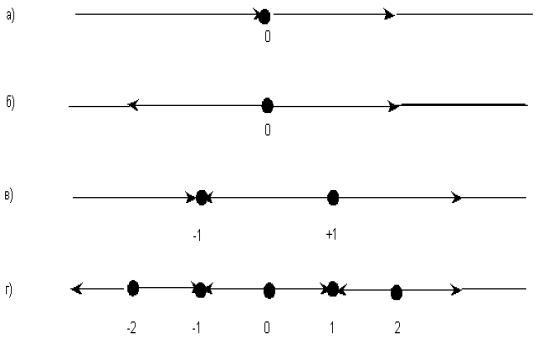
\includegraphics[
			width=\linewidth,
			height=3.3cm,
			keepaspectratio=false
			]{img/3_01}
			\vspace{-3mm} % Поднимает подпись
			\hspace*{4em} % Сдвигает подпись вправо
			{\small \centering Примеры фазовых траекторий}
		\end{minipage}
	\end{figure}
	
	\subsection{Линейные системы и их фазовые портреты}
	
	Система:
	\begin{equation}
		\frac{d x}{d t} = A x
	\end{equation}
	
	Точка $x = 0$ — очевидная точка равновесия. 
	\newline
	Пусть $\lambda_k$, $u_k$ - собственные значения и векторы матрицы $A$, а $U$ - матрица с векторами $u_k$ в столбцах.
	\vspace{-1.5em}
	\begin{align}
		A u_k &= \lambda_k u_k, \quad U = (u_1, u_2), \notag \\
		A U &= U \Lambda, \quad \Lambda = U^{-1} A U = \operatorname{diag}(\lambda_1, \lambda_2)
	\end{align}
	
	Замена $x = U y$ даёт:
	
	\begin{equation}
		\frac{d \mathbf{y}}{d t} = \Lambda \mathbf{y}, \quad \Lambda = \begin{pmatrix} \lambda_1 & 0 \\ 0 & \lambda_2 \end{pmatrix}
	\end{equation}
	
	Уравнения:
	\begin{equation}
		\frac{d y_1}{d t} = \lambda_1 y_1, \quad \frac{d y_2}{d t} = \lambda_2 y_2
	\end{equation}
	
	Решения:
	\begin{equation}
		y_1(t) = C_1 e^{\lambda_1 t}, \quad y_2(t) = C_2 e^{\lambda_2 t}
	\end{equation}
	
	\newpage
	Рассмотрим различные сочетания собственных значений:
	
	\begin{pinkbox}
		\subsection*{Вариант 1. Одного знака}
	\end{pinkbox}
	
	\begin{enumerate}
		\item $\lambda_1 < 0$, $\lambda_2 < 0$ (например, $\lambda_1 = -1$, $\lambda_2 = -2$):
		\begin{equation}
			y_1(t) = C_1 e^{-t}, \quad y_2(t) = C_2 e^{-2t}
		\end{equation}
		\vspace{-0.4em}
		$y_2(t) = C_3 y_1^2(t)$, $C_3 = \frac{C_2}{C_1^2}$ — \textbf{устойчивый узел} (парабола).
		\item $\lambda_1 > 0$, $\lambda_2 > 0$ (например, $\lambda_1 = 1$, $\lambda_2 = 2$):
		\begin{equation}
			y_1(t) = C_1 e^{t}, \quad y_2(t) = C_2 e^{2t}
		\end{equation}
		\vspace{-0.4em}
		$y_2(t) = C_3 y_1^2(t)$, $C_3 = \frac{C_2}{C_1^2}$ — \textbf{неустойчивый узел}.
	\end{enumerate}
	В обоих случаях при $C_1 = 0$ и $C_2 = 0$ получаем траектории на оси абсцисс или ординат
	\vspace{-0.5em}
	\begin{figure}[H]
		\centering
		\begin{minipage}[b]{0.49\linewidth}
			\centering
			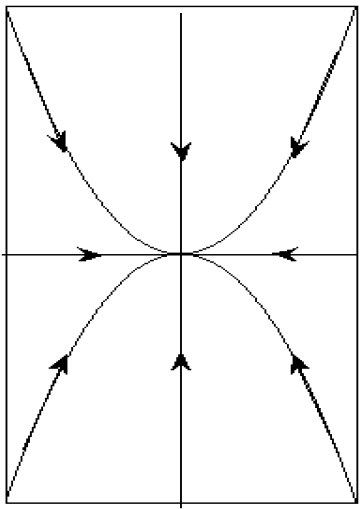
\includegraphics[width=0.5\linewidth]{img/3_02}
			\par
			\small Устойчивый узел
		\end{minipage}
		\hfill
		\begin{minipage}[b]{0.49\linewidth}
			\centering
			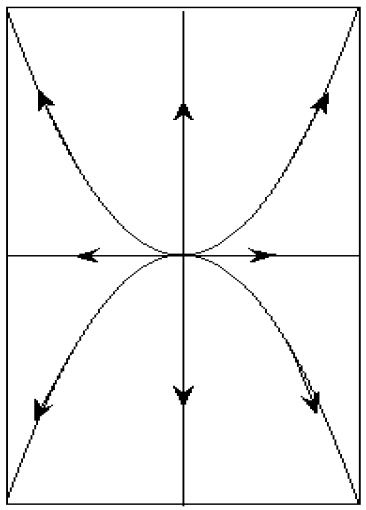
\includegraphics[width=0.5\linewidth]{img/3_03}
			\par
			\small Неустойчивый узел
		\end{minipage}
	\end{figure}
	
	\begin{pinkbox}
		\subsection*{Вариант 2. Разного знака}
	\end{pinkbox}
	
	$\lambda_1 > 0$, $\lambda_2 < 0$ (например, $\lambda_1 = 1$, $\lambda_2 = -1$):
	\newline
	\begin{equation}
		y_1(t) = C_1 e^{t}, \quad y_2(t) = C_2 e^{-t}
	\end{equation}
	$y_2(t) = \frac{C_3}{y_1(t)}$, $C_3 = C_1 \cdot C_2$ — гипербола (седло).
	\par
	\vspace{0.5em}
	при $C_1 = 0$ и $C_2 = 0$ получаем траектории на оси абсцисс или ординат
	
	\begin{figure}[H]
		\centering
		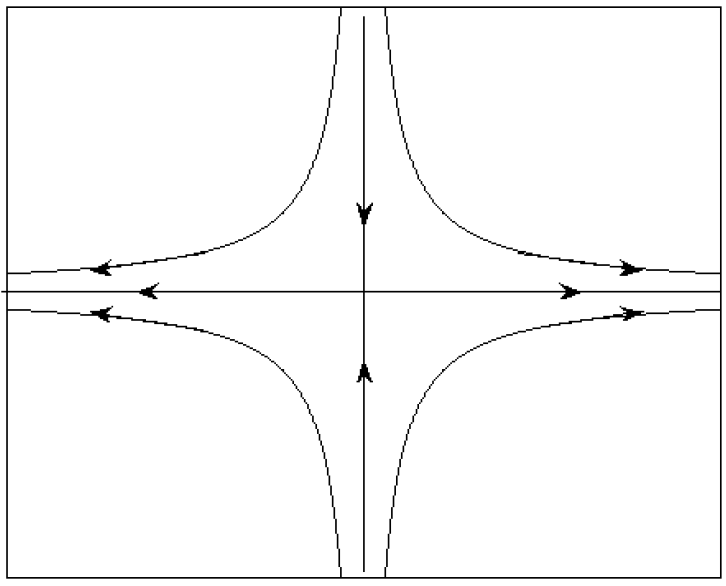
\includegraphics[width=0.4\textwidth, height=0.2\textheight]{img/3_04}
		\par
		\small Равновесие типа «седло»
	\end{figure}
	
	\begin{pinkbox}
		\subsection*{Вариант 3. Комплексно-сопряжённые}
	\end{pinkbox}
	
	$\lambda_{1,2} = \alpha \pm i \omega$:
	\begin{equation}
		y_1(t) = C_1 e^{\alpha t} \cos(\omega t), \quad y_2(t) = C_2 e^{\alpha t} \sin(\omega t)
	\end{equation}
	При $C_1 = C_2 = 1$:
	\begin{equation}
		y_1^2 + y_2^2 = e^{2 \alpha t}
	\end{equation}
	$\alpha < 0$ — устойчивый фокус, $\alpha > 0$ — неустойчивый фокус.
	
	\begin{figure}[H]
		\centering
		\begin{minipage}[b]{0.49\linewidth}
			\centering
			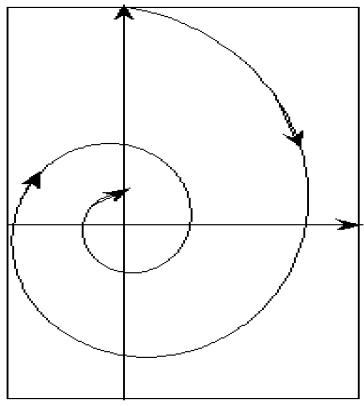
\includegraphics[width=0.7\linewidth]{img/3_05}
			\par
			\small Устойчивый фокус
		\end{minipage}
		\hfill
		\begin{minipage}[b]{0.49\linewidth}
			\centering
			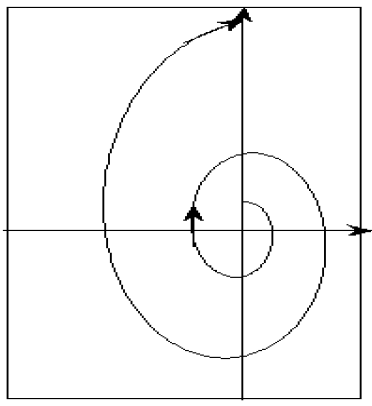
\includegraphics[width=0.7\linewidth]{img/3_06}
			\par
			\small Неустойчивый фокус
		\end{minipage}
	\end{figure}
	
	\subsection{Нелинейные системы}
	
	В малой окрестности точки равновесия нелинейную систему можно сколь угодно точно аппроксимировать линейной, поэтому поведение её решений соответствует типовым фазовым портретам.
	
\end{document}